\chapter{\label{chapter:vtmodel}A Virtualization model for embedded systems}

This chapter presents the virtualization model proposed by this dissertation. As discussed in Subsection \ref{section3:considerations}, the techniques currently applied for virtualization on embedded environments do not meet all requirements. Additionally, the evolution of the embedded processors is growing towards the usage of hardware support for virtualization. However, this is ongoing, and the next generations of embedded processors will support new hardware features for virtualization. Thus, the existing virtualization techniques for ES require continuous improvement and new approaches must be proposed. Based on the state-of-the-art for embedded virtualization, a set of important features were chosen as a guideline for the development of embedded virtualization models. Section \ref{section4:desirable} discusses these features. Section \ref{section:propose} presents the proposed virtualization model. The Embedded Systems Group (GSE) started to research embedded virtualization in 2010. Since then, another virtualization model was proposed by Aguiar \cite{aguiar2013}. Thus, Section \ref{section:vhh} compares the virtualization model presented in this dissertation to the model proposed by Aguiar \cite{aguiar2013}. Finally, Section \ref{section:final4} is the final considerations of this chapter. 

\section {Desirable Features for an Embedded Virtualization Model}
\label{section4:desirable}

This section states the important features for an embedded virtualization model. As explained before, real-time support on virtualized ESs has become an major concern, since all works presented in Chapter \ref{chapter:stateofart} have some support for real-time. However, these works still have different drawbacks. Widely adopted hypervisors like Xen and KVM (see Subsections \ref{section:xen} and \ref{section:kvm}) were designed for enterprise usage and do not scale well on some ESs because of their memory footprint. Solutions designed to target ESs, like SPUMONE, XtratuM and L4/Fiasco (see Sections \ref{section:spumone}, \ref{section:XtratuM} and \ref{subsection:fiasco}) have different constraints. For example,  SPUMONE does not provide spatial isolation, XtratuM was designed for critical systems, therefore it does not support GPOSs, and L4/Fiasco was designed for only single-core processors and it does not have proper real-time support. Moreover, the most of the hypervisors do not make use of the current hardware-assisted support present in the modern embedded processors. The only exception is the Xvisor (Section \ref{section:xvisor}), but its support is restrict to ARM processors. The research shows an increasing interest in emergent topics like hardware-assisted virtualization and security. Thus, it is essential to address these topics on a virtualization model. 

Based on the related works, there is not a consolidated approach for embedded virtualization. Additionally, due to the wide diversity of ES architectures and applications, there is not a single approach that can overcome all challenges at once. Nevertheless, more accurate techniques can be applied to build a hypervisor able to better address the virtualization needs on the most of ESs. Thus, this dissertation suggests a virtualization model that supports the following major features:

\begin{itemize}
\item \textbf{Hardware-assisted virtualization}: Considering that virtualization will be widely adopted for ESs shortly, the manufacturers will provide hardware-assisted virtualization for their embedded CPUs. The decreased fabrication cost of the embedded processors allowed for the adoption of hardware features for virtualization support. In fact, ARM and MIPS have already specified their  virtualization extensions as seen in \cite{armvt} and \cite{mipsvz}. Additionally, several manufacturers have released their virtualization platforms. Once the hardware supports a flexible set of features, hypervisor designers must decide what policy usage to adopt. As explained in Subsection \ref{subsection:hardware-assisted}, hardware-assisted virtualization allows more efficient and simpler hypervisors. The main advantages of the hardware-assisted virtualization are to speed-up hypervisor performance, save engineering costs and improve time to market.

\item \textbf{Multicore support}: Multicore processors are already widespread in ES platforms. When available, the hypervisor should ensure the proper support to obtain maximum performance. Additionally, migration of VCPUs between physical cores should be considered to allow load balancing. 

\item \textbf{Real-Time support}: Real-time is an intrinsic characteristic of embedded systems. The hypervisor should be predictable and ensure temporal isolation between GPOS and real-time applications. For multimedia purposes, soft real-time support is enough. Nevertheless, some ESs require accurate time constraints to run with GPOSs. For example, a smartphone system that must support a rich user graphical interface still needs to deal with the GSM stack \cite{appleton1998} time constraints. In this case, real-time support is desirable because it avoids the need for a second processor dedicated to the GSM stack.

\item \textbf{Coexistence of multiple GPOSs and Real-time instances}: A GPOS is highly desirable for certain ESs, such as smartphones and set-up boxes, due to its wide diversity of software. However, usually GPOSs have poor real-time responsiveness. In fact,the hypervisor must guarantee real-time instances that are executed with GPOSs. Additionally,  some virtualized platforms can require more than one GPOS at the same time. For example, in a virtualized network router that, for reliability reasons, the data plan must be isolated from the control plan. 

\item \textbf{Direct mapped and shared devices}: The current generation of embedded platforms designed for virtualization do not support I/O virtualization. Thus, when it is necessary to share a physical device, e.g. an Ethernet device, the hypervisor may use the para-virtualization technique. In this case, a device driver at hypervisor level serializes the access to the Ethernet device, and the guest OS implements a para-virtual device driver. However, aiming better performance, when device sharing is not desired, the hypervisor must map the device directly to the desired guest OS. Efficient implementation of directly mapped devices depends on the support of the processor's hardware (see Subsection \ref{subsection:interrupt}).

\item \textbf{Security}: The hypervisor must provide robust spatial isolation between VMs, i.e., a misbehavior in the guest OS should not affect the behavior of the other guest OSs or even the hypervisor. The goal of separation used for security purposes is to create and preserve a trusted operating environment for an embedded system. Separation is intended to prevent exploitable defects in one virtualized environment from propagating to adjacent virtual environments, or to the physical platform as a whole \cite{security-prpl}.

\item \textbf{Inter-VM communication}: A virtualized system is composed by a set of VMs. Possibly, these VMs will require some level of interaction between them. Also, some applications can require secure communication channels for sensitive information. Thus, an efficient and secure inter-VM communication mechanism must be available in the hypervisor.

\item \textbf{Lightweight virtualization layer}: Due to the resource constraints on ESs, the hypervisor layer must have a small memory footprint and induce the least amount of overhead possible. This requirement is intrinsically related to hardware-assisted virtualization. As explained in Section \ref{subsection:hardware-assisted}, greater hardware support simplifies hypervisor implementation and can improve performance.   
\end{itemize}

The design of an embedded hypervisor should consider this features. However, some are difficult to measure. For example, if the hypervisor is lightweight, it cannot be measured directly, but it can only be compared regarding the lines of code and memory footprint of similar hypervisors. Security is another feature that is hard to evaluate. The simplest way to evaluate security is to consider if the hypervisor ensures spatial isolation or separation between VMs. However,  critical systems may require formal proof. Other system characteristics are directly measured based on responsiveness, memory and time overhead. Section \ref{section:propose} presents the proposed virtualization model that is flexible enough to accommodate these features. 



\section{Model Overview}
\label{section:propose}

An innovative virtualization model was proposed based on the desired features described in the Section \ref{section4:desirable}. As a result, an implementation of this model is presented in the Chapter \ref{chapter:implementation}. Thus, this section describes the proposed virtualization model. However, there are two considerations about this model:

\begin{enumerate}
  \item The model does not try to impose or improve the real-time capabilities of non real-time entities, like a GPOS. Instead, it provides mechanisms for GPOSs and real-time entities coexist and;
  
  \item The model was not designed to be a pure full-virtualization model. Instead, it was designed to support full-virtualization of the CPU and use the para-virtualization concept for other services, such as communication and shared devices.
\end{enumerate}

Many hypervisor solutions for ESs try to improve the real-time responsiveness of GPOSs in virtualized environments. For example, different authors propose to apply techniques to improve the Linux real-time responsiveness when virtualized in KVM or Xen (see sections \ref{subsection:kvmproposals} and \ref{subsubsection:xenproposals}). However, the proposed model avoids the utilization of GPOSs as real-time instances. Instead, it allows real-time services to be directly scheduled by the hypervisor, see Subsection \ref{subsection4:realtime}. Additionally, the model provides full-virtualization based on the hardware-assistance of the CPU. Other peripherals may require para-virtualization techniques, see Subsection \ref{subsection4:services}.  

Figure \ref{fig:virtmodel} depicts the proposed model. At the hardware level, it uses a bus-based homogeneous MPSoC along with shared memory. The first software layer is the the hypervisor, which is responsible for the creation and management of each VM. It also provides a logic arrangement for associating the VM with its VCPUs. Moreover, the hypervisor controls the memory space of each VM for memory isolation. Thus, this model describes a hypervisor type 1, as explained in Subsection \ref{subsection:hypertypes}. Type 1 hypervisors usually requires lower footprint then type 2 ones, since they does not require an underline OS. 

\begin{figure}[!hbtp]
\centering
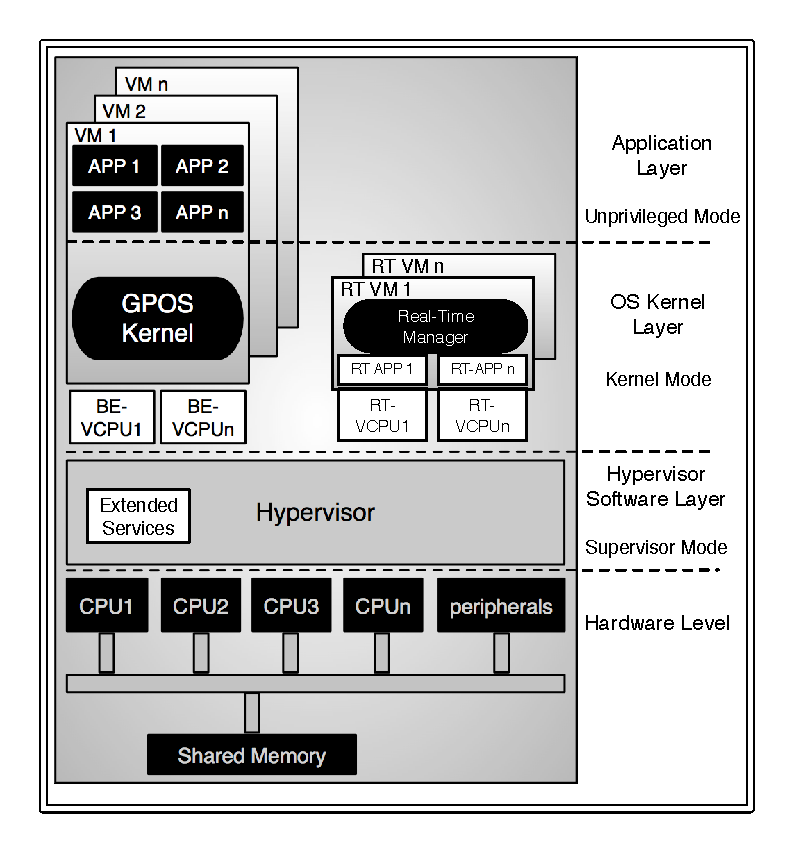
\includegraphics[width=.45\textwidth]{./chapter4/figures/hypervisormodel}
\caption{Overall view of the proposed virtualization model.}
\label{fig:virtmodel}
\end{figure}

The GPOSs are mapped onto best-effort VCPUs while real-time instances are mapped onto real-time VCPUs, as further explained in Subsection \ref{subsection:flex}. The model takes advantage of the processor's additional privilege levels (see Subsection \ref{subsubsection2:privelege}) to provide spatial isolation between hypervisor and guests. Additionally,  unlike virtualization models that do not utilize the additional privilege levels scheme, the proposed model can provide spatial isolation between the guest kernel and guest applications. Therefore, the hypervisor is protected from the actions of malicious or misbehaving guest OSs and the guest OSs are protected from their applications. 

The model provides additional features, called extended services, that expand the virtualization platform functionalities. See Subsection \ref{subsection4:services} for more details. Additionally, for better temporal isolation, the model proposes the adoption of the RT-VM, which maps real-time services onto RT-VCPUs, as explained in Subsection \ref{subsection4:realtime}. Finally, direct communication among VMs is possible using shared memory areas or message passing mechanisms can be implemented using the hypervisor as a communication arbiter, which is explained in detail in Subsection \ref{subsection4:comm}.


\subsection{The Flexible Scheduling Mapping}
\label{subsection:flex}

Figure \ref{fig:mappingmodel} shows the possible flexible mapping and the partitioning model for virtualized architectures based in the proposed model. To perform temporal isolation between VMs, the hypervisor specifies two different kinds of VCPUs:  best-effort VCPUs (BE-VCPUs) and real-time VCPUs (RT-VCPUs). RT-VCPUs have priority over BE-VCPUs and follow the policy of a real-time scheduling algorithm. BE-VCPUs are scheduled by a best-effort scheduler algorithm that is invoked when there are not RT-VCPUs ready to execute. Additionally, the BE-VCPUs can migrate among physical cores, i.e., when a CPU becomes idle the scheduler will choose the next BE-VCPU ready to run in a global queue. The migration of RT-VCPUs depends on the real-time scheduler algorithm adopted. Due to time constraints, a real-time scheduler algorithm for multicore processors must be carefully designed, as proposed by \cite{saranya2015} and \cite{vigeant2015}. This model is flexible enough to accommodate different combinations of real-time and best-effort scheduler algorithms, which is an implementation decision. 

\begin{figure}[!hbtp]
\centering
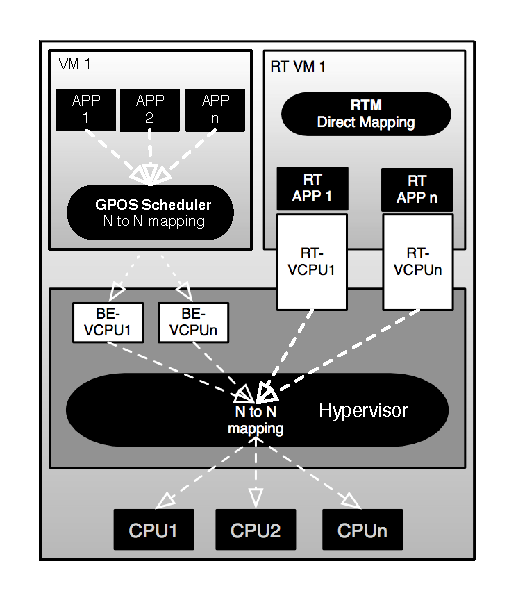
\includegraphics[width=0.45\textwidth]{./chapter4/figures/flexiblemapping}
\caption{Flexible mapping for multiprocessor embedded systems with real-time support.}
\label{fig:mappingmodel}
\end{figure}

A multiprocessing GPOS may have several BE-VCPUs available, and its scheduler is responsible for mapping the task among BE-VCPUs according to its policies. At the hypervisor level, the best-effort scheduler algorithm will map a BE-VCPU to the next idle CPU. This arrangement enables an N-to-N mapping of task over BE-VCPUs and BE-VCPUs over CPUs. 


\subsection{Extended Services}
\label{subsection4:services}

The model suggests the implementation of the para-virtualization concept to provide extended services to the guest OSs. Extend services are useful to expand the virtualization platform functionalities, i.e., to implement functions that does not exist in a pure fully-virtualized system. Hypercalls are widely used in para-virtualization based approaches, where the guest OS needs to be modified to invoke hypercalls instead of using privileged instructions. However, this work uses  full-virtualization with a hardware-assisted technique, where the guest OS does not need to be modified for virtualization purposes.  Yet it must use hypercalls to take advantage of the  extended services, e.g., real-time services and communication among VMs. 

The model suggests a minimal set of extended services. However, an implementation can add services for different purposes as necessary. Table \ref{table:hypercalls} resumes the extended services available through hypercalls. Altogether, six different hypercalls are supported and may be implemented by a guest OS when needed. The services are divided into three different groups:

\begin{itemize}
    \item VM identification composed by a hypercall that returns a unique VM identification number issued by the hypervisor.
    \item RT-VCPU management is composed by a group of three hypercalls responsible to manage the RT-VCPUs. Using this hypercalls the guest OS can create, launch or delete  real-time services.  
    \item Communication services are composed of two hypercalls designed for communication purposes.
\end{itemize}


\begin{table}[!hbtp]
\caption{Hypercalls as extended services.}
\centering
\begin{tabular}{l l l}
\hline\hline \\
\textbf{Extended Service} & \textbf{Hypercall} & \textbf{Description} \\ 
\hline \\
VM identification & HCALL\_INFO\_GET\_ID  & Return the VM ID number  \\
\hline
\multirow{3}{*}{RT-VCPU  Management} & 
    HCALL\_RT\_CREATE\_APP & RT application Instantiation  \\
    & HCALL\_RT\_LAUNCH\_APP & RT application launch  \\
    & HCALL\_RT\_DELETE\_APP & RT application delete \\
    \hline
\multirow{2}{*}{Communication Services} & 
     HCALL\_IPC\_SEND\_MSG  & Send messages \\ 
    & HCALL\_IPC\_RECV\_MSG & Receive messages \\ \hline
\end{tabular}
\label{table:hypercalls} 
\end{table}

The utilization of the hypercalls for management  of the RT-VCPUs is better explained in Subsection \ref{subsection4:realtime}. The extended services proposed in Table \ref{table:hypercalls} are supported by the hypervisor implementation presented in Chapter \ref{chapter:implementation}.

\subsection{Real-time Aspects}
\label{subsection4:realtime}

To deal with real-time constraints, a special VM called RT-VM was designed to provide a robust temporal isolation between real-time services and GPOSs. The RT-VM does not support RTOSs. Instead, it implements what is  called a Real-Time Manager (RTM), which supports communication facilities and basic user libraries. The RTM can map its tasks directly to RT-VCPUs in the hypervisor scheduler, i.e., it does not implement a scheduler on its level avoiding the hierarchical scheduling problem and improving performance. The real-time services must be registered during the RT-VM initialization calling the HCALL\_RT\_CREATE\_APP hypercall. After the registration, the real-time services are available in the system and they can be started/stopped by the guests using the hypercalls HCALL\_RT\_LAU\-NCH\_APP and HCALL\_RT\_DELETE\_APP. 

RTM may or not provide spatial isolation between tasks. Providing spatial isolation means the implementation of virtual memory support on the RTM, which may impact in the real-time responsiveness. Nevertheless, if spatial isolation between different services is desired, more than one RT-VM can be instantiated. When a developer is interested in taking advantage of real-time in this model, he must implement its real-time service using the RTM API.

The RT-VCPUs are scheduled by a real-time algorithm, e.g., EDF, which has priority over the best-effort scheduling algorithm. To keep the RT-VCPUs in a global queue (allowing migration) or in a local queue per CPU is a implementation decision. As described in Subsection \ref{subsection:flex}, an implementation for multi-core processor using a global queue and allowing CPU migration must be carefully designed to guarantee temporal isolation. Additionally, critical systems require schedulability analysis to guarantee system resource availability during RT-VCPU admission. Finally, during the execution of a RT-VCPU, interrupts sent to BE-VCPUs may or not be postponed in order  to increase temporal isolation, see Section \ref{section5:interrupt} about interrupt delivery policies.

\subsubsection{Schedulability Analysis for Real-time Services}

As explained, the real-time services are available in the RT-VM, and they can be started/stopped by the guest OSs. An important concern about this scheme is how to deal with concurrent real-time services that can be started asynchronously. For example, a set of real-time services available in a RT-VM may not be schedulable altogether. Thus, some of the real-time services may not be accepted for execution when a guest OS requires it due to unavailable CPU time. This is especially critical for systems where the non-execution of a service may cause safety concerns. 

The model does not specify mechanisms for schedulability analysis or any other approach to avoid the schedulability problem. In fact, to determine the schedulability of a task set, the real-time scheduling algorithm and the real-time scheduling parameters must be known. However, the model allows for different real-time algorithms making the schedulability analysis dependant of implementation. Finally, the simpler approach for a hypervisor based on this model to avoid schedulability problems is to guarantee the schedulability of the set of real-time services available in the system. For this, two approaches can be take: 

\begin{itemize}
    \item The development team performs a schedulability analysis;
    \item The hypervisor implements its own schedulability test, that is performed during its initialization. 
\end{itemize}

Both approaches can be used together. If the development team fails in their schedulability analysis, the hypervisor can detect the problem during the system's initialization, since the RT-VM must register its services at boot time using the hypercall HCALL\_R\-T\_CREATE\_APP. It is important to highlight that both approaches work only for real-time services implemented at design time. However, the model does not permit to install new real-time services in runtime. The hypervisor implementation presented in Chapter \ref{chapter:implementation} implements the schedulability test to the EDF scheduler algorithm. 

\subsection{Communication Model}
\label{subsection4:comm}

Inter-VM communication capabilities must be implemented as part of the extended services, i.e., using hypercalls. However, the model does not impose any specific communication mechanism. Instead, this decision is made by the developer. For example, for better performance, the designers may choose to implement direct communication between VMs using memory sharing. Or, if the major concern is security, the designers may choose to implement a message exchange mechanism using the hypervisor as a communication arbiter. The model's implementation presented in Section \ref{chapter:implementation} provides communication between VMs using the hypervisor as a manager.  

Inter-device communication, i.e., communication of the virtualized platform with external devices is desirable in modern ESs. The proposed model is flexible enough to support typical socket style \cite{tanenbaum2011} communication among VMs. Thus, the hypervisor may implement a network layer in order to route Internet Protocol (IP)  datagrams \cite{tanenbaum2011} between VMs. Still, when communication with the external world is desired, the hypervisor may virtualize a network adapter providing network capabilities to the platform. Nevertheless, in the embedded system context, the socket communication scheme can be expensive in terms of system overhead, therefore message passing may be preferable.

\section{Comparison with the Virtual Hellfire Hypervisor (VHH)}
\label{section:vhh}

In 2010, the GSE group started to research virtualization for embedded systems. Aguiar \cite{aguiar2013}, proposed an embedded virtualization model and a hypervisor implementation in 2013. The resulting hypervisor was called Virtual Hellfire Hypervisor (VHH). This section discusses the main differences between the virtualization model proposed by Aguiar and the model presented in this dissertation. 

Figure \ref{fig:vhhmodel} presents the VHH's virtualization model. Similar to the model proposed in this dissertation, the VHH model assumes a bus-based homogeneous MPSoC along with shared memory. On top of the CPUs, it executes the hypervisor, which is responsible for the creation and management of each Application Domain Unit (ADU). The ADU is a logical arrangement responsible for associating the guest OS with its VCPUs. Moreover, each ADU has its own memory space controlled by the hypervisor to provide memory isolation. Applications can be mapped on best-effort (non-real-time) and real-time VCPUs according to their needs in an ADU. The guest OS is responsible for instantiating RT-VCPUs for each real-time application it wishes to execute.

\begin{figure}[!hbtp]
\centering
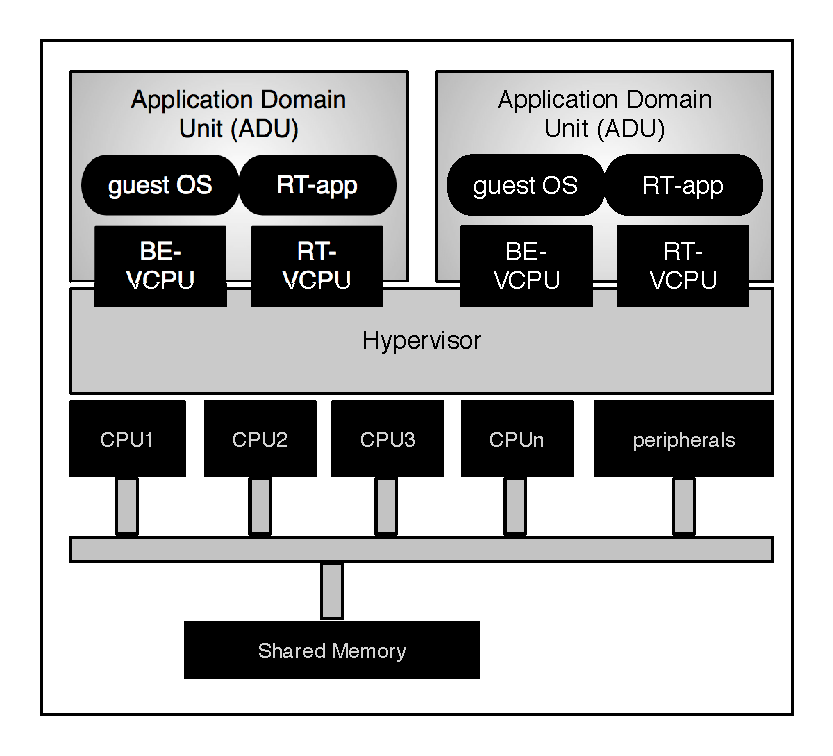
\includegraphics[width=0.50\textwidth]{./chapter4/figures/vhhModel}
\caption{Virtual Hellfire Hypervisor's virtualization model.}
\label{fig:vhhmodel}
\end{figure}

The VHH's model was designed to be compatible with the existing embedded processors that were available at the time it was developed, see Section \ref{section2:future}. Thus, the resulting model does not support essential hardware features to meet security and performance providing full-virtualization without hardware-assistance. A side effect is the absence of spatial isolation between the guest OS's kernel and user modes. Without additional processor privilege levels, the entire guest OS must execute in user-mode. In addition, all privileged instructions must be handled by the hypervisor. Thus, the model can only be used when the processor meets the Popek and Goldberg requirements (see Subsection \ref{subsection:vz-requirements}). 

Aguiar's model provides weak temporal isolation between real-time and non-real-time applications since it does not provide spatial isolation between BE-VCPUs and RT-VCPUs. Figure \ref{fig:vhhmodel} shows that BE-VCPUs and RT-VCPUs coexist in ADUs. Sharing memory space is advantageous for software stack sharing and communication performance. This means that a GPOS could instantiate RT-VCPUs that share all its software stack and communicate using shared memory. However, this approach has one major drawback. A RT-VCPU may be prevented from executing because a BE-VCPU is holding a shared lock causing a priority inversion. The model proposed in this work, implements spatial isolation between real-time and best-effort VCPUs to provide stronger temporal isolation between them.

The VHH's model was implemented in the 4Kc MIPS processor. This implementation required the modification of the target processor to allow virtualization of the MIPS's exception vector \cite{moratelli2015}. As the processor's core was modified the hypervisor could not be evaluated in a hardware platform, thus only OVSim \cite{ovp2015} simulations were performed. Also, the resulting implementation has performance issues as shown in \cite{aguiar2013}. Despite the fact that full-virtualization avoids the need for guest OS modifications, the absence of hardware-assistance forces the hypervisor to intervene constantly in the execution of the guest OS. The hypervisor handles all system interrupts routing them to the destined guest OS. VHH uses the trap-and-emulate strategy to deal with privileged instructions. Additionally, memory mapped devices use a similar strategy. When the guest OS tries to access a protected memory address, the hypervisor intervenes checking if it is a valid address to the guest OS, if so, the hypervisor proceeds to emulate the operation. The model proposed in this dissertation uses hardware-assistance to avoid excessive hypervisor intervention. Finally, guest OSs are allowed to access memory mapped devices directly and interrupts targeted to guests can be directly routed. 


\section{Final Considerations}
\label{section:final4}

The proposed embedded virtualization model was designed to take advantage of the current technologies available in the embedded processor families. These technologies allow for full-virtualization of the CPU, but they do not support efficient I/O virtualization. Despite the advantage of avoiding guest modifications, experience with the VHH has shown that full-virtualization without proper hardware support results in excessive overhead. Thus, this model avoids full-virtualization for hardware subsets without proper hardware-assisted virtualization. As a result, the proposed model implements a hybrid approach, which provides full-virtualization for the CPU and para-virtualization for I/O devices. Additionally, a list of major features for embedded virtualization was determined and the model was designed to support them. For example, spatial isolation among VMs is guarantied based on hardware support while temporal isolation is provided by BE and RT-VCPUs. Moreover, the extended services concept uses para-virtualization to allow inter-VM communication and real-time service management.

The hierarchical scheduling problem is avoided by the introduction of the RT-VM that maps real-time services directly onto RT-VCPUs. The flexible scheduling mapping proposed may cause the LHP (Subsection \ref{subsection:holder}) because a multiprocessing OS with concurrent VCPUs may be preempted while holding a spinlock. However, the LHP is not directly addressed in the model, since this problem requires different approaches depending of the scheduling algorithm implemented. But, it can be avoided with different approaches. For example, the real-time services proposed in this model does not implement spinlocks. Thus, they will not be subjected to the LHP. Additionally, single-core processors where the hypervisor maps each VM to a single VCPU does not suffer from the LHP.

The model proposed in this dissertation strengthens the hypothesis that is possible to have an embedded lightweight hypervisor capable of supporting the major embedded virtualization requisites Moreover, hardware-assisted virtualization is important to achieve low footprint and high performance. 

%hypothesis that a definition of an embedded virtualization model using hardware-assisted virtualization would result in a hypervisor capable of supporting the key required features for embedded virtualization. 

